\documentclass[]{report}
\usepackage{amsmath}
\usepackage{amssymb}
\usepackage[english]{babel}
\usepackage[utf8]{inputenc}
\usepackage[T1]{fontenc}
\usepackage{euler}

\usepackage[inner=0cm,outer=0cm,top=0.1cm,bottom=0cm,paperwidth=4.6cm,paperheight=4.6cm]{geometry}

\usepackage{tikz,pgfplots}
\usetikzlibrary{positioning}
\usetikzlibrary{decorations.pathmorphing}

\begin{document}
\centering
	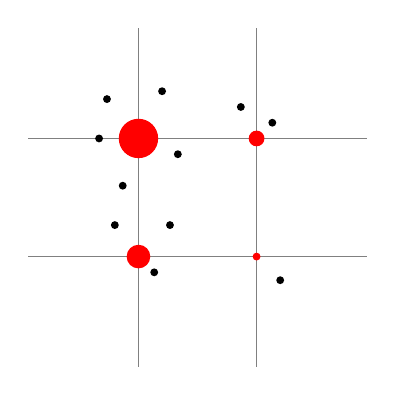
\begin{tikzpicture}
		\draw[gray,step=1.5] (0.1,0.1) grid (4.4,4.4);
		\fill[fill=red] (1.5,3) circle (0.25);
		\fill[fill=red] (3,1.5) circle (0.05);
		\fill[fill=red] (1.5,1.5) circle (0.15);
		\fill[fill=red] (3,3) circle (0.1);

		\fill[fill=black] (1, 3) circle (0.05);
		\fill[fill=black] (2, 2.8) circle (0.05);
		\fill[fill=black] (1.1, 3.5) circle (0.05);
		\fill[fill=black] (1.3, 2.4) circle (0.05);
		\fill[fill=black] (1.8, 3.6) circle (0.05);

		\fill[fill=black] (1.2, 1.9) circle (0.05);
		\fill[fill=black] (1.7, 1.3) circle (0.05);
		\fill[fill=black] (1.9, 1.9) circle (0.05);

		\fill[fill=black] (3.2,3.2) circle (0.05);
		\fill[fill=black] (2.8,3.4) circle (0.05);

		\fill[fill=black] (3.3,1.2) circle (0.05);
	\end{tikzpicture}
\end{document}
	